
%(BEGIN_QUESTION)
% Copyright 2012, Tony R. Kuphaldt, released under the Creative Commons Attribution License (v 1.0)
% This means you may do almost anything with this work of mine, so long as you give me proper credit

In this process, sulfur-laden water is ``stripped'' of sulfur compounds by the addition of hot steam.  A level control system is supposed to maintain a constant level of liquid at the bottom of the stripping tower, but it seems to have a problem:

$$\includegraphics[width=15.5cm]{i0007rx01.eps}$$

\filbreak

Here is what the trend recording from LR-12b looks like during the time an operator placed the controller in manual mode and then back to automatic mode:

$$\includegraphics[width=15.5cm]{i01902x01.eps}$$

A fellow technician tells you he thinks the controller is over-tuned (having too much gain).  The operator, who just did the manual-mode test, disagrees.  Based on the information seen in the trend, what do you think the source of the oscillation is, and how would you go about testing your hypothesis?

\underbar{file i01902}
%(END_QUESTION)





%(BEGIN_ANSWER)

This oscillation is clearly not the result of an over-tuned controller, because it persists even when the controller is in manual mode.  The source must be coming from somewhere else in the process.

\vskip 10pt

At this point in time, it would be a good thing to note the frequency of this oscillation, and begin searching for anything that could cause the level to go up and down at this frequency, or perhaps something that could ``fool'' level transmitter LT-12 into thinking the level is oscillating at this frequency.  If the frequency is relatively high, local machine vibration could be the cause of it.  This hypothesis makes a lot of sense, based on the fact that the controller's action in automatic mode doesn't seem to be correcting the oscillations at all: the oscillation amplitude seems to remain unchanged between automatic and manual modes.  This is what we might expect from a vibration-induced oscillation, where the frequency of the oscillation is much faster than the liquid level can possible change, and therefore faster than the level control system can physically compensate.

%(END_ANSWER)





%(BEGIN_NOTES)

\vskip 20pt \vbox{\hrule \hbox{\strut \vrule{} {\bf Virtual Troubleshooting} \vrule} \hrule}

This question is a good candidate for a ``Virtual Troubleshooting'' exercise.  Presenting the diagram to students, you first imagine in your own mind a particular fault in the system.  Then, you present one or more symptoms of that fault (something noticeable by an operator or other user of the system).  Students then propose various diagnostic tests to perform on this system to identify the nature and location of the fault, as though they were technicians trying to troubleshoot the problem.  Your job is to tell them what the result(s) would be for each of the proposed diagnostic tests, documenting those results where all the students can see.

During and after the exercise, it is good to ask students follow-up questions such as:

\begin{itemize}
\item{} What does the result of the last diagnostic test tell you about the fault?
\item{} Suppose the results of the last diagnostic test were different.  What then would that result tell you about the fault?
\item{} Is the last diagnostic test the best one we could do?
\item{} What would be the ideal order of tests, to diagnose the problem in as few steps as possible?
\end{itemize}

%INDEX% Basics, control loop troubleshooting (realistic P&ID shown)
%INDEX% Process: sour water stripping tower (realistic P&ID shown)
%INDEX% Process troubleshooting: diagnosing problem via trend recording

%(END_NOTES)

